\chapter{\overviewofoptions}\label{chapter:overview}

This chapter will be expanded into a complete reference for the
various \topspin\ options.  At the moment, every option is listed, but some of the descriptions are minimal.

\section{Online help}

Running \topspin\ with a single argument, \texttt{help}, displays a list of command-line switches and configuration file options for which
short help messages can be generated.

Running \topspin\ with two arguments, \texttt{help <option>}, where \texttt{<option>} is one of the options for which help is available, displays
a short message describing the function of the option.

\section{Command-line options}\label{sec:overview:commandline}

\subsection{\texttt{-check}}

Apply this switch to just type-check a specification.  Type checking will be symmetry-aware: the checker will report errors if the specification
contains features which will cause symmetry detection to fail, \eg arithmetic on \texttt{pid} variables, or absence of an \texttt{init} process.

When using the \texttt{-check} option it is not necessary to use \inline{config.txt}, as the typechecking process does not depend on other tools
or options.

\subsection{\texttt{-detect}}

Apply this switch to type-check and detect symmetry for a specification, but \emph{not} apply symmetry reduction.  \topspin\ will report the
symmetries it computes, indicating whether there are problems in detecting symmetry.  This option can be useful if you want to find out the extent to
which symmetry is present in a model, but not actually do symmetry reduction.

Because this option does not require the output of symmetry reduction algorithms, \topspin\ will detect symmetries for specifications containing features
which are not supported for symmetry reduction, \eg a \texttt{never} claim.  The idea here is that these features could, in principle, be supported
fully, and determining whether symmetry is present may still be of interest.

\subsection{\texttt{-relaxedarrayindexing}}\label{sec:overview:commandline:relaxedarray}

\topspin\ is based on the \etch\ typechecker, which tries to help modellers improve the quality of their specifications by performing relatively
strict type-checking.  In particular, \etch\ does not allow an array to be indexed by an expression with a numeric type larger than \texttt{byte}.
This is because the maximum size of an array in Promela is 255, which is also the largest \texttt{byte} value.

So, for example, the following code snippet will cause a type error:

\begin{lstlisting}
mtype myArray[12];
int x;
x = ...;
myArray[x] = ...
\end{lstlisting}

\noindent due to the fact that \texttt{myArray} has been indexed by \texttt{x}, which has type \texttt{int}.

Sometimes, in practice, it is useful to index an array using a larger type than \texttt{byte}, \eg\ so that a non-\texttt{byte} value like
-1 can be used to represent a null index.  For this reason, \topspin\ can be passed the \texttt{-relaxedarrayindexing} command-line option,
instructing the tool to allow indexing of arrays by expressions of \emph{any} numeric type.

Note that the efficiency of a verification model can be improved by using smaller types: an \texttt{int} takes up more state-vector space than
a \texttt{byte}, so the user should consider re-modelling their specification to use \texttt{byte} variables to index arrays where possible.

\subsection{\texttt{-relaxedassignment}}\label{sec:overview:commandline:relaxedassign}

As with array indexing, \topspin\ performs strict typechecking of numeric assignments by default, and rejects assignments from an expression
of a ``large'' integer type (\eg \texttt{short}) to a ``smaller'' integer type (\eg \texttt{bit}).  This is to prevent arithmetic overflow
where possible.

So, for example, the following code snippet will cause a type error:

\begin{lstlisting}
byte k;
k = -1;
\end{lstlisting}

\noindent due to the fact that \texttt{-1} has type \texttt{short}, which is a larger type than \texttt{byte}.

Because \spin\ is not as strict as this, practical examples may rely on this kind of assignment.  For this reason, specifying
\texttt{-relaxedassignment} on the command line tells \topspin\ to allow a variable of any numeric type to be assigned the result
of an expression of any numeric type.

As in \secref{overview:commandline:relaxedarray}, note that where possible, smaller numeric types should be used for reasons of efficiency.  If you find you need the
\texttt{-relaxedassignment} option then consider whether you could refactor your specification to use smaller types, removing the need
for this option and reducing the size of the state-vector.

\section{Mandatory configuration file options}

\subsection{\texttt{saucy}}

String option specifying path to the \saucy\ program.  This option must be set by the user.

\subsection{\texttt{common}}

String option specifying path to the \texttt{Common} directory, which is part of the \topspin\ distribution.  This option must be set by the user.

\subsection{\texttt{gap}}

String option specifying path to the \gap\ program.  This option must be set by the user.

\section{Configuration file options for symmetry detection}


\subsection{\texttt{explain}}

\topspin\ detects symmetry by finding the \emph{static channel diagram} for the input specification, computing its symmetries, and checking these
symmetries for validity against the Promela specification.  Some symmetries may not be valid: \topspin\ will try to compute the largest valid set
of static channel diagram symmetries.

If you have written a specification which you expect to be symmetric, but for which \topspin\ reports invalid symmetries, it may be interesting
to inspect the reason for this invalidity: it could indicate a typo in the specification, a misunderstanding on the part of the user, or a limitation
of \topspin.

Setting \texttt{explain} to a positive integer $n$ tells \topspin\ to output explanations for the first $n$ invalid symmetries.  An ``explanation''
for an invalid symmetry $\alpha$ consists of a pair of text files, one called \texttt{$m$\_original.txt}, the
other \texttt{$m$\_permuted.txt} (where $m<n$).  The \emph{original}
file shows the input specification before $\alpha$ is applied, then shows the specification after \emph{normalization} has taken place.  The
\emph{permuted} file shows the input specification after $\alpha$ has been applied, then shows the permuted specification after normalization.
\topspin\ regards a symmetry as valid if these normalized specifications are the same, so obviously they will not be identical for $\alpha$.

The two text files can be compared with a diff tool (\eg\ the excellent WinMerge\footnote{http://www.winmerge.org/}).  Looking at the differences
in the normalized parts should be instructive as to why the given symmetry is not valid.

By way of example, here is a mutual exclusion specification with five processes:

\begin{lstlisting}
mtype = {N,T,C}
mtype st[6]=N

proctype user() {
  do
    :: d_step { st[_pid]==N -> st[_pid]=T }
    :: d_step { st[_pid]==T &&
        (st[1]!=C && st[2]!=C && st[1]!=C && st[4]!=C && st[5]!=C)
    -> st[_pid]=C
       }
    :: d_step { st[_pid]==C -> st[_pid]=N }
  od
}

init {
  atomic {
    run user();
    run user();
    run user();
    run user();
    run user();
  }
}
\end{lstlisting}

Running \topspin\ on this example, in verbose mode and with \texttt{explain=1}, produces output including the following:

\begin{lstlisting}
Saucy computed the following generators for Aut(SCD(P)):
   Aut(SCD(P)) = <(3 2),(2 1),(3 4),(5 4)>
--------------------------------------
Computing valid generators:
    (3 2) : not valid
        generating explanation in files 0_original.txt and 0_permuted.txt
    (2 1) : not valid
    (3 4) : not valid
    (5 4) : valid
--------------------------------------
\end{lstlisting}

The tool has determined that the symmetry $(3\;2)$ which swaps \texttt{user} processes 3 and 2 is not valid, and has written an explanation to the files
\inline{0_original.txt} and \inline{0_permuted.txt}.

\begin{figure}
\center
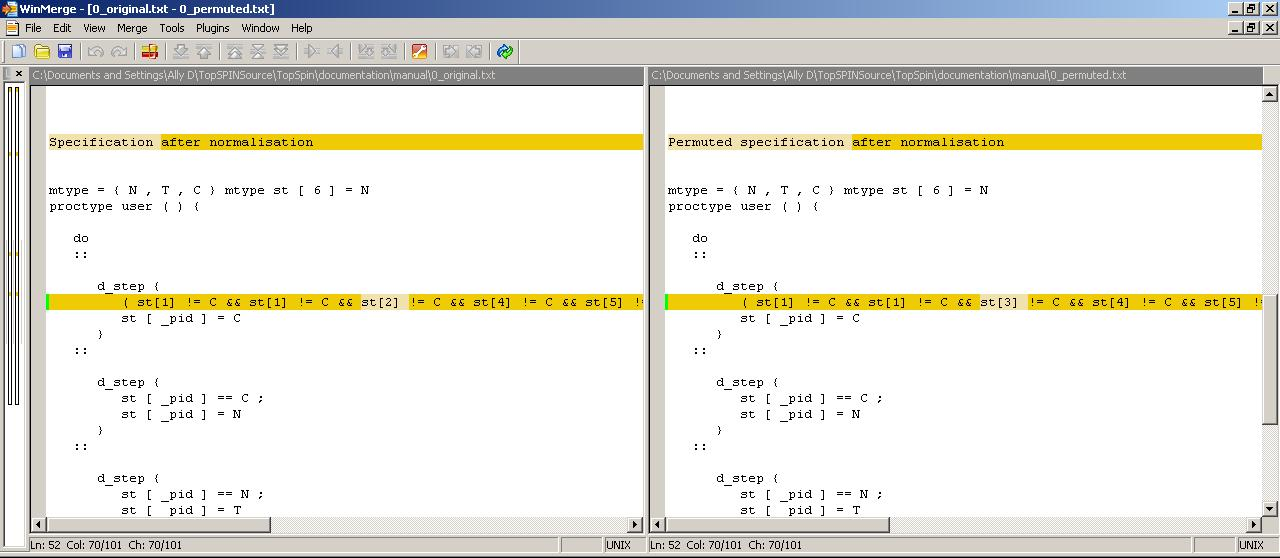
\includegraphics[scale=0.46]{explain.jpg}\caption{Comparing text files output by the \texttt{explain} option to see why symmetry $(3\;2)$ is not valid.}\label{fig:explain}
\end{figure}


\figref{explain} shows the results of comparing these files with WinMerge.  This should alert the user to the fact that the operand \inline{st[1] != C} appears
twice in the highlighted boolean expression: this is clearly a mistake -- one of these operands should be changed to \inline{st[2] != C} to restore full
symmetry and presumably correct the model.

This illustrates the idea that presence of symmetry can actually be a correctness requirement in its own right.

\noindent\textbf{Default value: } 0, \ie no explanations will be given.

\subsection{\texttt{timebound}}

When detecting symmetry, \topspin\ may use a coset search to try to improve upon the initially computed group of symmetries.  This search
can be time-consuming on particular examples.  The \texttt{timebound} integer option limits the length of time dedicated to this search to a maximum
number of seconds.

\noindent\textbf{Default value: } 0, which is used to specify that the coset search should be unbounded.

\subsection{\texttt{conjugates}}

If the coset search is taking a long time, it is sometimes possible to speed things up by picking a number of candidate symmetries
at random, finding the \emph{conjugate} of each known valid generator by these random elements, and then testing the conjugates for
validity.  This is based on the practical observation that valid symmetries are often conjugate to other valid symmetries.  The
\texttt{conjugates} integer option is used to specify how many conjugates to use.

\noindent\textbf{Default value: } 0.  If symmetry detection is slow, try 5 conjugates.

\subsection{\texttt{symmetryfile}}

Sometimes \topspin\ is unable to automatically detect symmetry from an input specification even though the user knows that symmetry exists.
In this case, it is possible to specify a file containing generators for a symmetry group.  The name of this file is specified via the
\texttt{symmetryfile} option.  If \texttt{symmetryfile} is set, \topspin\ will not attempt automatic symmetry detection, and will use the
given group of symmetries for symmetry reduction.

\noindent\textbf{Default value: } no file specified, automatic symmetry detection will be attempted..

\section{Configuration file options for symmetry reduction}\label{sec:overview:symmetryreductionconfig}

\subsection{\texttt{strategy}}

String option specifying the strategy to use for symmetry reduction.  Options are: fast, enumerate, hillclimbing, segment, flatten, exactmarkers, approxmarkers.

\noindent\textbf{Default value: } fast.

\subsection{\texttt{transpositions}}

Boolean option stating whether to apply group elements as transpositions.

\noindent\textbf{Default value: } true.

\subsection{\texttt{stabiliserchain}}

Boolean option stating whether to use a stabiliser chain for enumeration.

\noindent\textbf{Default value: } true.

\subsection{\texttt{vectorise}}

Boolean option stating whether to use vector SIMD instructions for symmetry reduction.  The nature of the resulting
vector code depends on the \texttt{target} configuration file option (see \secref{overview:symmetryreductionconfig:target}).

\noindent\textbf{Default value: } false.

\subsection{\texttt{parallelise}}

Boolean option stating whether to parallelise symmetry reduction using pthreads.

\noindent\textbf{Default value: } false.

\subsection{\texttt{cores}}

Integer option stating the number of cores available for parallel symmetry reduction.

\noindent\textbf{Default value: } 1.

\subsection{\texttt{target}}\label{sec:overview:symmetryreductionconfig:target}

String option specifying the target to use for vector and parallel symmetry reduction.  Options are: PC, CELL, POWERPC.

\noindent\textbf{Default value: } not set by default.

\section{Configuration file options for usability}

\subsection{\texttt{profile}}

Profile the performance of TopSPIN?

\noindent\textbf{Default value: } false.

\subsection{\texttt{verbose}}

Display progress of TopSPIN in detail?

\noindent\textbf{Default value: } false.

\subsection{\texttt{quiet}}

Suppress non-vital output?

\noindent\textbf{Default value: } false.
